\documentclass[11pt, oneside]{article}   	% use "amsart" instead of "article" for AMSLaTeX format
\usepackage{geometry}                		% See geometry.pdf to learn the layout options. There are lots.
\geometry{letterpaper}                   		% ... or a4paper or a5paper or ... 
%\geometry{landscape}                		% Activate for for rotated page geometry
%\usepackage[parfill]{parskip}    		% Activate to begin paragraphs with an empty line rather than an indent
\usepackage{graphicx}				% Use pdf, png, jpg, or eps� with pdflatex; use eps in DVI mode
								% TeX will automatically convert eps --> pdf in pdflatex		
\usepackage{amssymb}
\usepackage{amsmath}
\usepackage{parskip}
\usepackage{color}
\usepackage{hyperref}

\title{Power series}
%\author{The Author}
%\section{}
%\subsection*{}
\date{}							% Activate to display a given date or no date

\graphicspath{{/Users/telliott_admin/Dropbox/Tex/png/}}
% \begin{center} 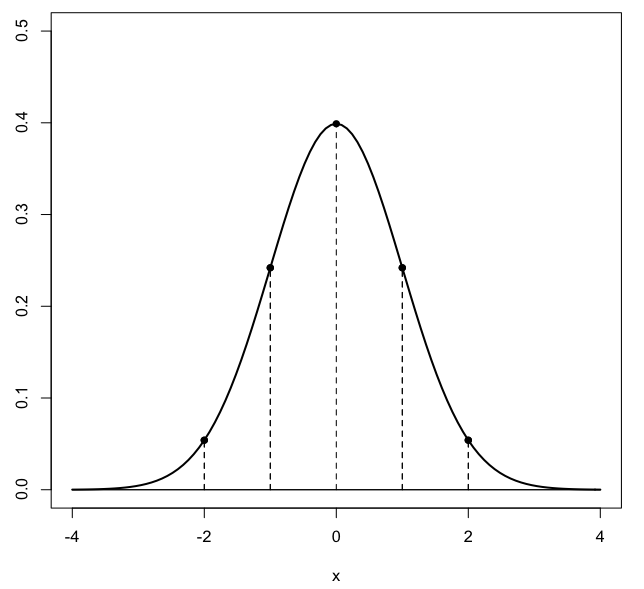
\includegraphics [scale=0.4] {gauss3.png} \end{center}
\begin{document}
\maketitle
\Large
Kharkar says that if $f$ is analytic over a domain then within a disk $\{z: |z - z_0| < R \}$ contained in that domain, it has a power series valid in the disk with the formula
\[ \sum_{k=0}^{\infty} a_k \ (z-z_0)^k \]
and that the coefficients are given by
\[ a_k = \frac{1}{2 \pi i} \int_{\gamma} \frac{f(z)}{(z -z_0)^{k+1}} \ dz \]
where $\gamma$ is the circle with radius $r$ and
\[ | z - z_0 | < r < R \]

Note, however, that the coefficients are also given by
\[ a_k = \frac{1}{k!} \ f^{(k)} (z_0) \]

\end{document} 